\section{Numerical Solutions for Diff Eq}
\subsection{a}
$$
x_1 = \theta
$$
$$
x_2 = \dot{\theta}
$$
$$
\dot{x_1} = \dot{\theta} = x_2 = \int{\dot{x_2}} = \dfrac{g}{L}cos(x_1)  + C
$$
$$
\dot{x_2} = \ddot{\theta} = -\dfrac{g}{L}sin\theta =  -\dfrac{g}{L}sin(x_1)
$$

\subsection{e}

\begin{itemize}
\item 'pend' represents the name of the diff eq being solved
\item '[0, 10]' the time span/range this simulation is run over
\item '[0; 1]' the initial condition of the state 
\end{itemize}

\subsection{f + g}
\begin{figure}[htbp]
   \centering
   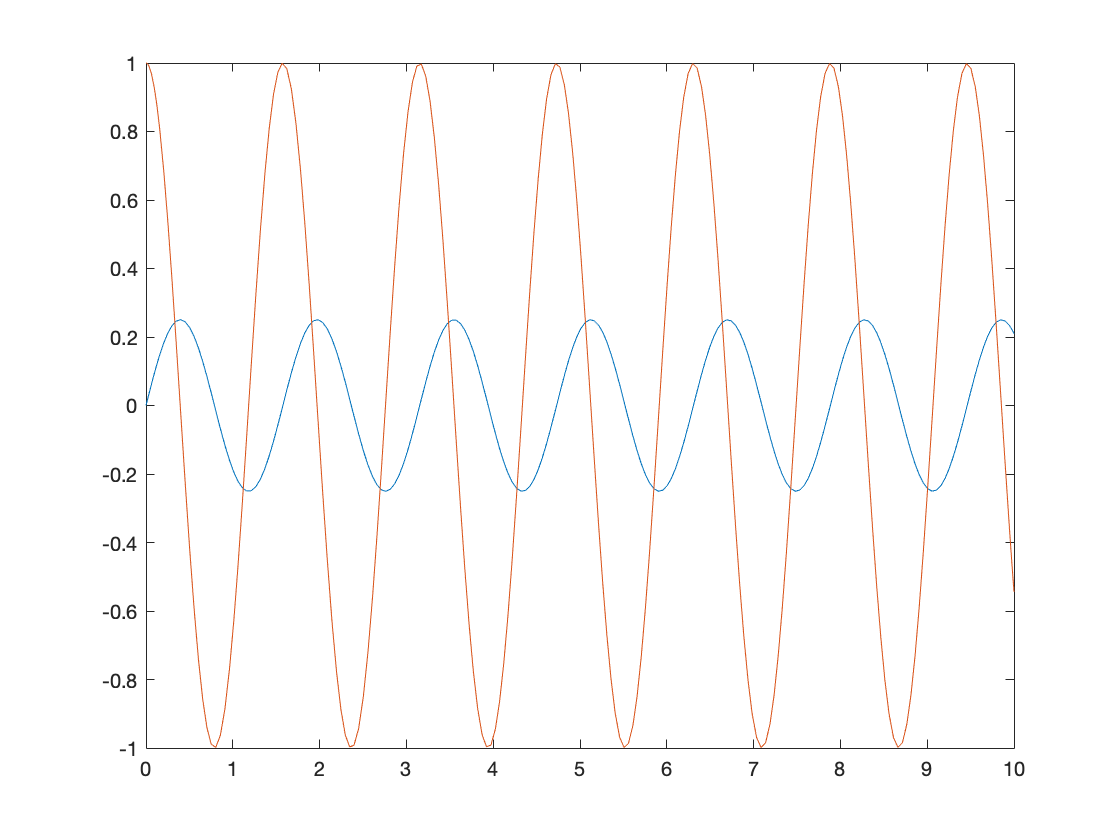
\includegraphics[width=\textwidth]{figs/pend.png}% requires the graphicx package
   \caption{Orange: xdot(1), Blue: xdot(2)}
   \label{fig:pend}
\end{figure}
See fig. \ref{fig:pend}.

\subsection{h}
\subsection{f + g}
\begin{figure}[htbp]
   \centering
   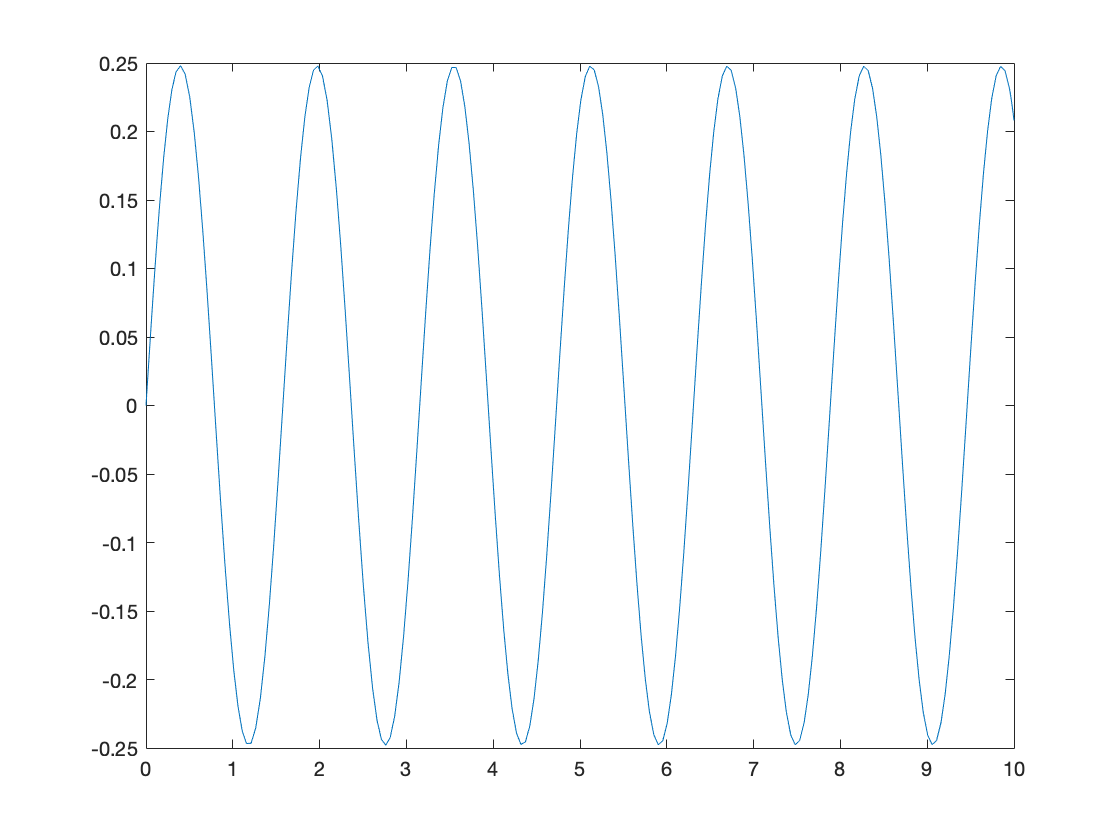
\includegraphics[width=\textwidth]{figs/pend_y.png}% requires the graphicx package
   \caption{Y component given angle over time. Result should be scaled by L. }
   \label{fig:pend_y}
\end{figure}

See fig. \ref{fig:pend_y}.